\section*{CERN guide, S'Cool Lab teacher, Finance Club admin, Boxing Club coach}

It has been a great pleasure to stay at CERN for four years. From the bottom of my heart, I want to thank my adviser and my HEP group for this opportunity. I have exploited all the possible areas of science, outreach, fun, and joy available at CERN. Well, almost all, and I know it is ridiculous, but here, in Gen\`eve, I have not yet tried skiing...

I have been an official CERN guide, giving people tours to the Antimatter Decelerator, the ATLAS control room, the Low Energy Ion Ring complex, the Proton Synchrotron, the LHC control room, the Data Centre, the SM18 facility (a world-leading magnet test facility for testing magnets and instrumentation at low temperature and high currents), and the Alpha Magnetic Spectrometer control room. The audience ranged from middle school kids to emeritus professors of science. 

Also, I have been a teacher at the S'Cool Lab, where high school students have a chance to come to CERN and build a real experimental setup at this ``cool'' scientific laboratory and then conduct an experiment on their own. 

For more than a year I have been an administrative managing officer at the CERN Finance Club. I was responsible for inviting top professionals from finance and FinTech companies to give talks at our club. I started the ``quant group'' and was the first to optimize our portfolio of stocks using Monte Carlo methods and minimization techniques. Needless to say, that would not have been possible if I had not learned those tools first in High Energy Physics!

Last but not least, thank you to my friends from the CERN Powerlifting Club who introduced me to the Boxing Club. There is where I met most of my CMS and ATLAS friends. I have been training people with the goal to improve their health. As a side effect, some picked up self-defense, others had fun and found themselves truly addicted to this combination of hard work and laughter. A few people journeyed into the world of intelligent boxing, which is not about power, but about strategy and outworking the opponent \ref{outreach}. 



\begin{figure}[h]
     \includegraphics[width=0.54\textwidth]{uni_of_geneva}
     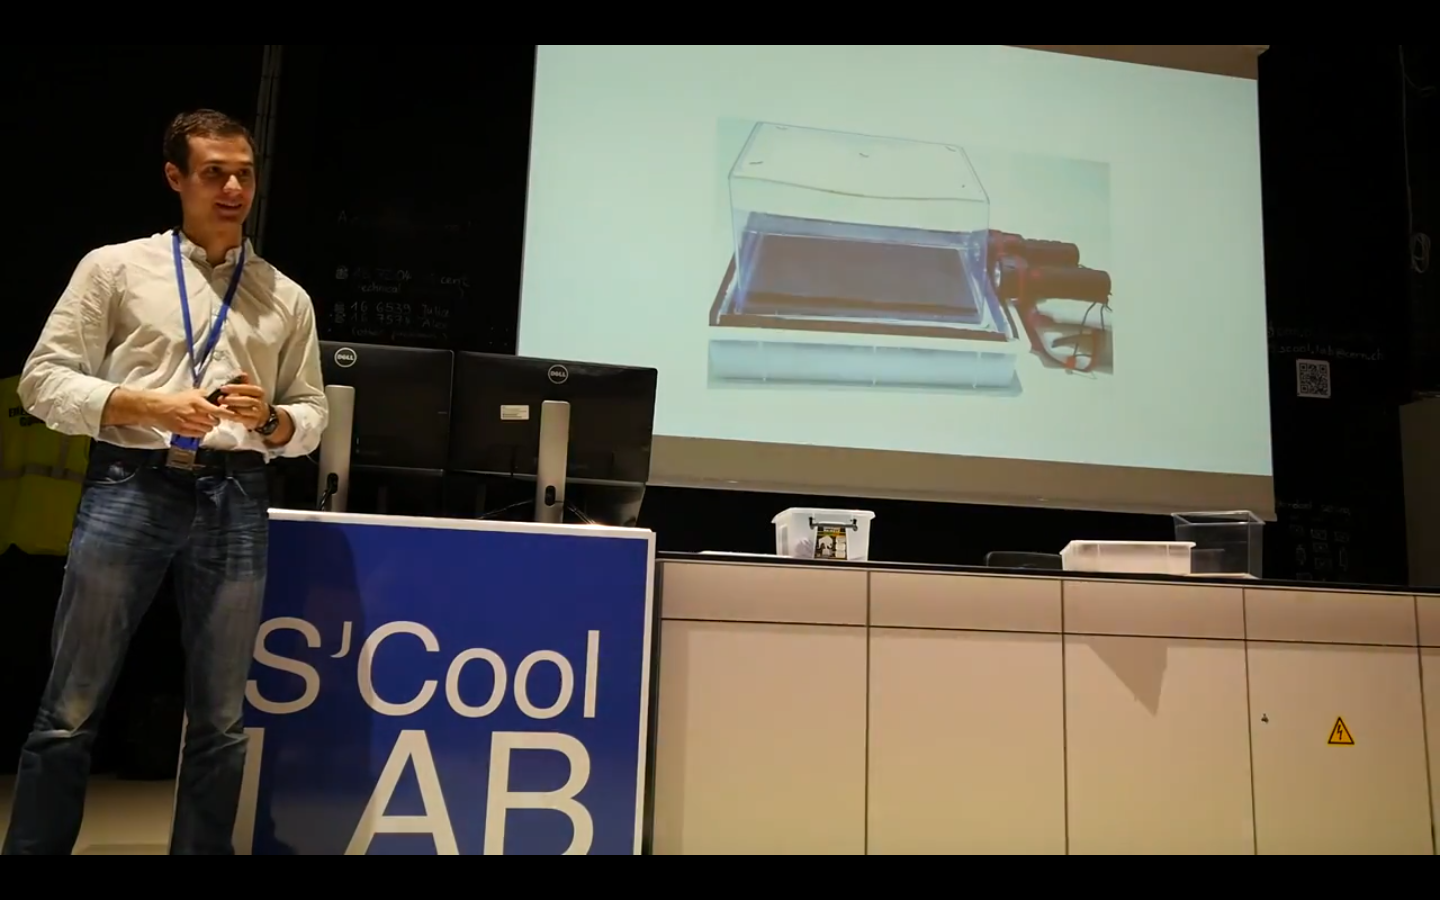
\includegraphics[width=0.54\textwidth]{scoollab3.png}\\
     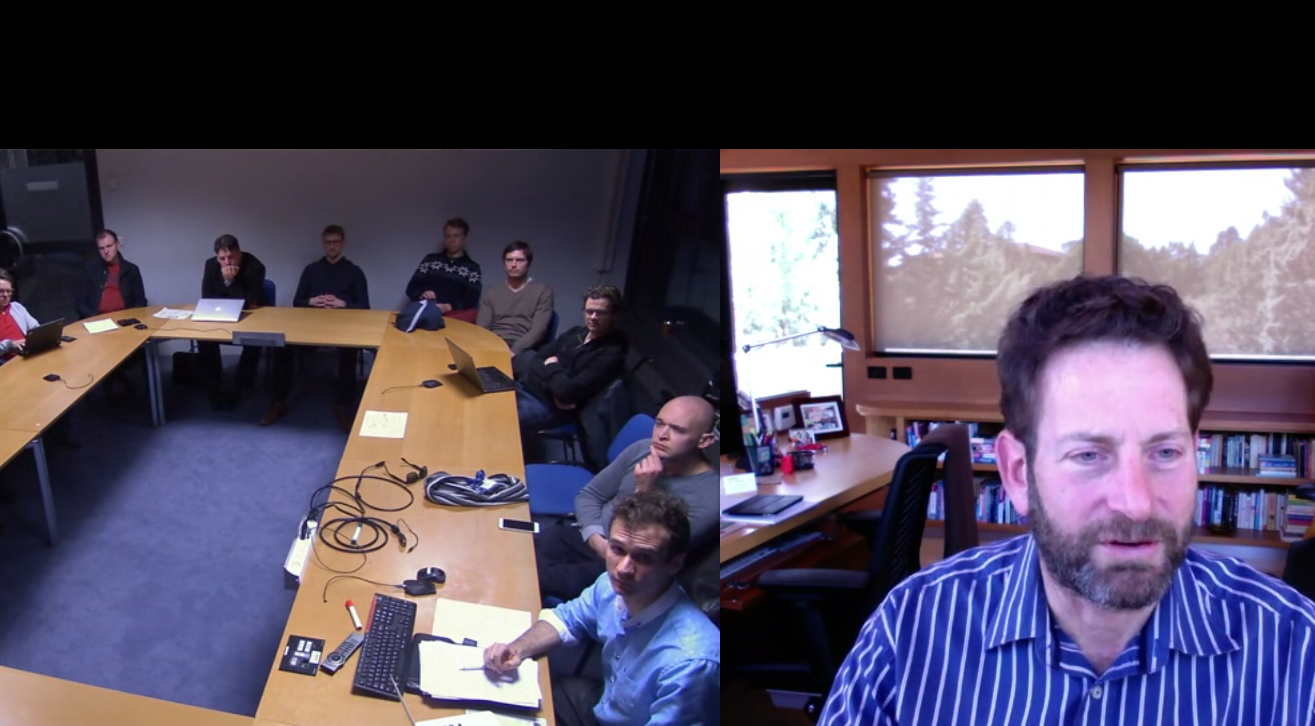
\includegraphics[width=0.54\textwidth]{finance1.png}
     \includegraphics[width=0.54\textwidth]{finance2.jpg}\\
     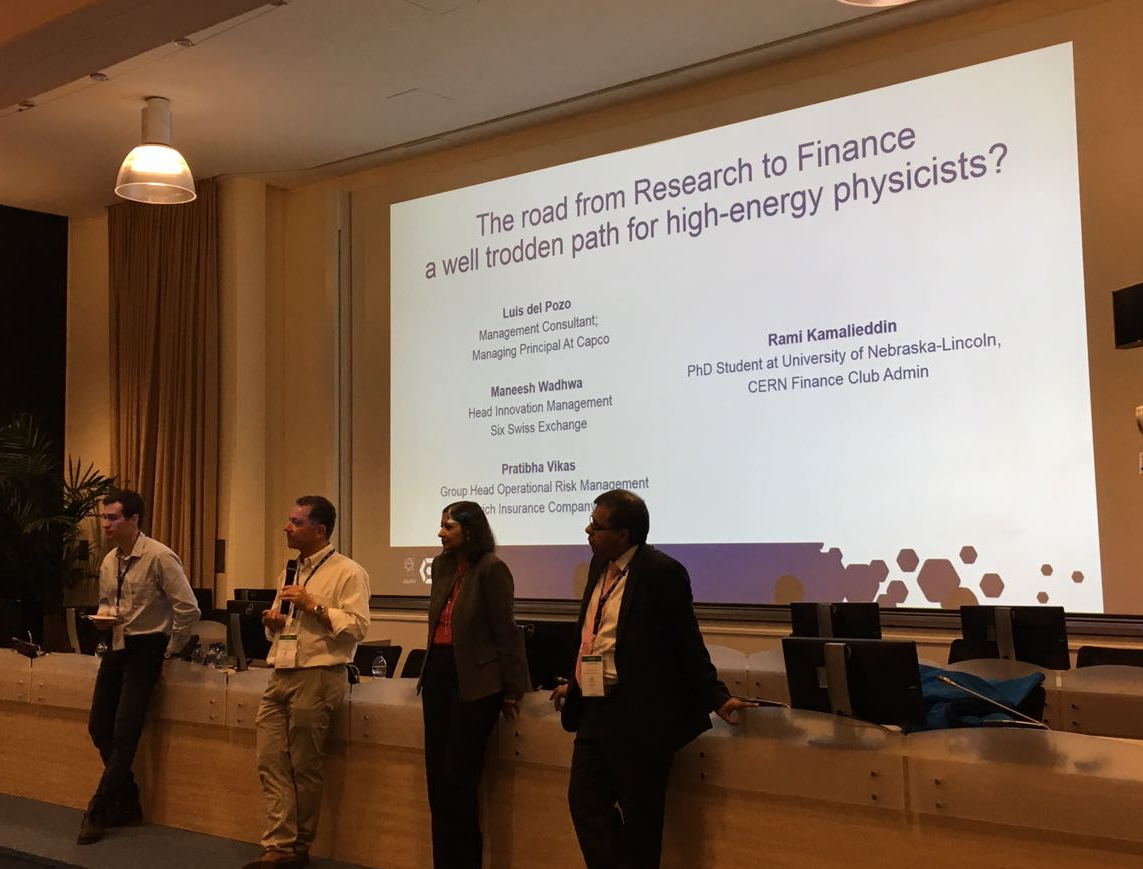
\includegraphics[width=0.54\textwidth]{finance3}
     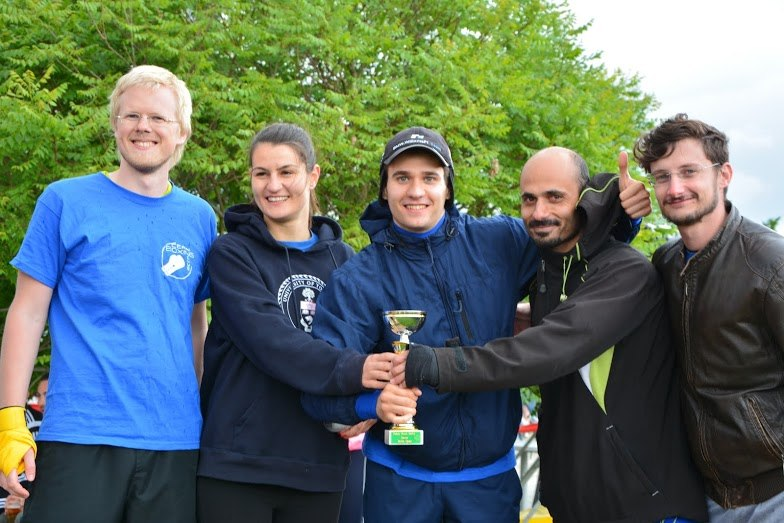
\includegraphics[width=0.54\textwidth]{boxing1.jpg}\\  
     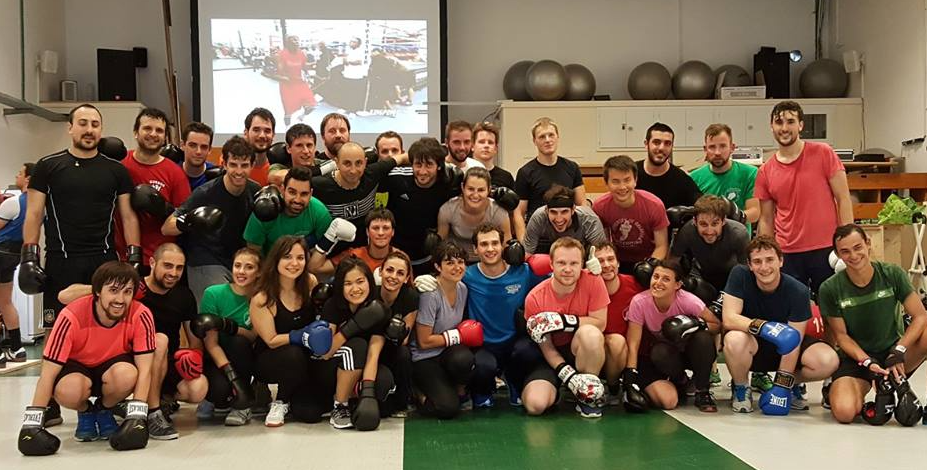
\includegraphics[width=0.54\textwidth]{boxing2}
     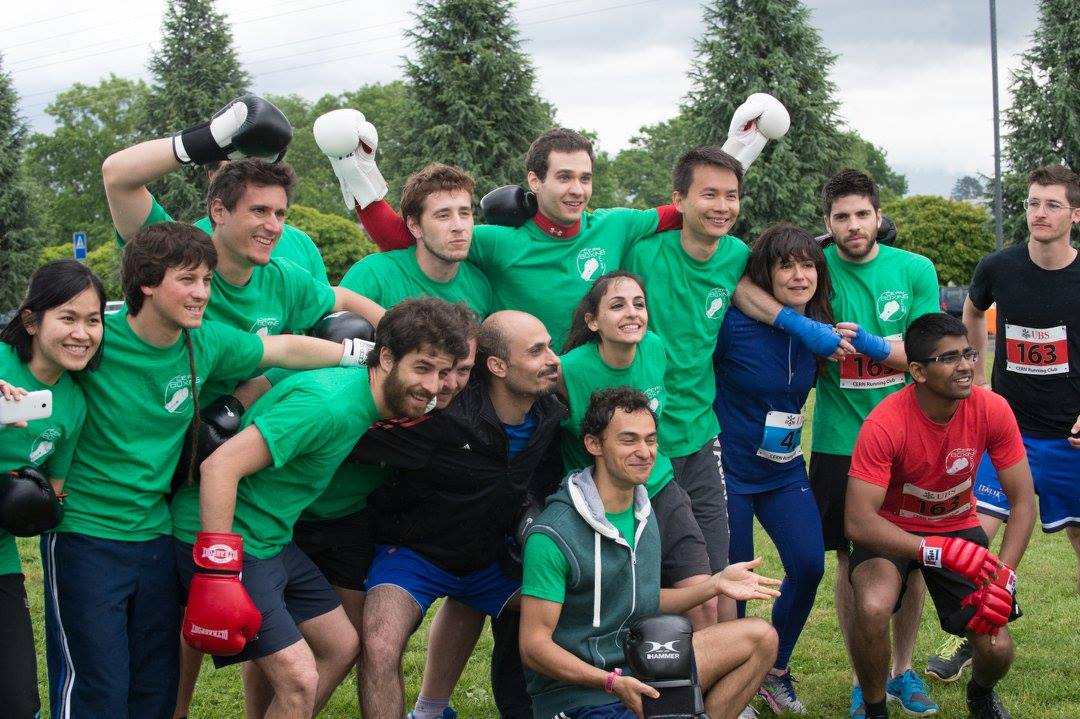
\includegraphics[width=0.54\textwidth]{boxing4.jpg}\\
    \caption{ Top row: visit at SM18 and S'Cool lab. Second row: invited talks at the Finance Club. Third row: moderator at the CERN Alumni Collisions and CERN Relay Race trophy. Bottom row: Boxing Club.}
 \label{outreach}
 \end{figure}


\iffalse

\fi

